%
\documentclass[journal]{IEEEtran}



\usepackage{amsfonts,latexsym}

\ifx\pdfoutput\undefined
\usepackage{graphicx}
\else
\usepackage[pdftex]{graphicx}
\fi

\usepackage{epstopdf}
\usepackage{amssymb}
\usepackage{amsmath}

\usepackage{multirow}
\usepackage{subfigure}


\usepackage{algorithm}
\usepackage{algpseudocode}



% correct bad hyphenation here
\hyphenation{op-tical net-works semi-conduc-tor}


\newtheorem{proposition}{Proposition}[section]
\newtheorem{observation}{Observation}[section]
\newtheorem{definition}{Definition}[section]


\begin{document}

\title{Title}
%
%
% author names and IEEE memberships
% note positions of commas and nonbreaking spaces ( ~ ) LaTeX will not break
% a structure at a ~ so this keeps an author's name from being broken across
% two lines.
% use \thanks{} to gain access to the first footnote area
% a separate \thanks must be used for each paragraph as LaTeX2e's \thanks
% was not built to handle multiple paragraphs
%

\author{ }

%\author{Michael~Shell,~\IEEEmembership{Member,~IEEE,}
%        and~Jane~Doe,~\IEEEmembership{Life~Fellow,~IEEE}% <-this % stops a space
%\thanks{M. Shell is with the Department of Electrical and Computer Engineering, Georgia Institute of Technology, Atlanta, GA, 30332 USA.}% <-this % stops a space
%\thanks{J. Doe and J. Doe are with Anonymous University.}% <-this % stops a space
%\thanks{Manuscript received April 19, 2005; revised December 27, 2012.}}

% note the % following the last \IEEEmembership and also \thanks - 
% these prevent an unwanted space from occurring between the last author name
% and the end of the author line. i.e., if you had this:
% 
% \author{....lastname \thanks{...} \thanks{...} }
%                     ^------------^------------^----Do not want these spaces!
%
% a space would be appended to the last name and could cause every name on that
% line to be shifted left slightly. This is one of those "LaTeX things". For
% instance, "\textbf{A} \textbf{B}" will typeset as "A B" not "AB". To get
% "AB" then you have to do: "\textbf{A}\textbf{B}"
% \thanks is no different in this regard, so shield the last } of each \thanks
% that ends a line with a % and do not let a space in before the next \thanks.
% Spaces after \IEEEmembership other than the last one are OK (and needed) as
% you are supposed to have spaces between the names. For what it is worth,
% this is a minor point as most people would not even notice if the said evil
% space somehow managed to creep in.



% The paper headers
\markboth{Journal name,~Vol.~xx, No.~x, December~2014}%
{Shell \MakeLowercase{\textit{et al.}}: Bare Demo of IEEEtran.cls for Journals}




% make the title area
\maketitle

\begin{abstract}

\end{abstract}

\begin{IEEEkeywords}
Keywords
\end{IEEEkeywords}






% For peer review papers, you can put extra information on the cover
% page as needed:
% \ifCLASSOPTIONpeerreview
% \begin{center} \bfseries EDICS Category: 3-BBND \end{center}
% \fi
%
% For peerreview papers, this IEEEtran command inserts a page break and
% creates the second title. It will be ignored for other modes.
\IEEEpeerreviewmaketitle



\section{Introduction}
This paper is collocated into the reconfigurable computing context. An important problem into the reconfigurable computing is to analyse the error propagation when the circuit ``under test'' is setted with values of the frequency too high or in disagree with the values of the delay. The paper investigates the propagation of the error caused by a timing violation into a digital online multiplier. \\

...................\\

This work starts from the results obtained in a previus work on the Radix-2 Digit-parallel Online Multiplier (see \cite{onlinearith}).\\
 In \cite{onlinearith} the autors have provided methodologies to implement a parallel version of the online multiplier and they have proposed a probabilistic model describing the propagations of the error caused by timing violation conditions. They also backed up the models with experimental results from an image processing application demostrating that this novel design methodology can lead to substantial performance benefits compared to the design method using conventional arithmetic. The purpose of this paper is to provide a numerical model estimating the error on the online multiplier and a model to estimate the probability of timing violation in order to provide an ``a priori'' estimation for the error expectation for different values of the circuit parameters (frequency, number of digits, online delay, etc).  \\
In this paper we provide a formal model of the Overclocking Error for the radix-2 digit-parallel Online Multiplier. We also proved a mathematical '``support'' to the experimental results obtained in  \cite{onlinearith} and, in particular, we estimate the expectation of the overclocking error for these results. We provide a model describing the probablity of timing violation as ``chain start probability'' and ``chain rule probability'' representing the probability that a chain starts during the operation and the probability that a chain starts $\&$ perpetuals for a fixed number of digits, respectively.  \\














\section{Background: Online Arithmetic}\label{Sec:Background}
\subsection{Key Features of Online Arithmetic}

Online arithmetic has been widely used in numerous applications such as signal processing and control algorithms~\cite{Online_FPGADSP,Online_Control}. Online arithmetic was originally designed for digit serial operation, as illustrated in Fig.~\ref{Fig:OnlineDataFlow}. It can be seen that in order to generate the first output digit, $\delta$ digits of inputs are required, where $\delta$ is called the ``online delay''. Normally $\delta$ a small constant, which is independent of the precision. For ease of discussion, for the rest of this paper, the input data is assumed to be fixed point numbers in the range $(-1,1)$. Based on this premise, the online representation of $N$-digit operands and result at iteration $j$ are given by (\ref{Eq:Online_Operands}), where $j\in[-\delta,N-1]$ and $r$ denotes the radix~\cite{Ercegovac_Book}.

\begin{figure}[tbp]
  \centering
  \includegraphics[width=.48\textwidth]{./Figures/OnlineArithmetic_DataFlow.pdf}
  %\vspace{-4ex}
  \caption{Dataflow in digit-serial online arithmetic, in which both inputs and outputs are processed from the MSD to the LSD. $\delta$ denotes the online delay.}
  %\vspace{-1ex}
  \label{Fig:OnlineDataFlow}
\end{figure}
%
\begin{eqnarray}\label{Eq:Online_Operands}
\footnotesize
  X_{[j]}=\sum_{i=1}^{j+\delta}x_ir^{-i},~Y_{[j]}=\sum_{i=1}^{j+\delta}y_ir^{-i},~Z_{[j]}=\sum_{i=1}^{j}z_ir^{-i}
\normalsize
\end{eqnarray}

MSD first operation is possible only if a redundant number system is used. Normally there are two most commonly used redundant number representations: carry-save (CS)~\cite{CSadder}  and signed-digit (SD)~\cite{RedundantNumber}. With SD representation, each digit is represented using a redundant digit set $\{-a,\cdots,-1,0,1,\cdots,a\}$ where $a\in[r/2,r-1]$. In comparison, the standard non-redundant representation only uses a digit set $\{0,\cdots,r-1\}$. Thus a standard number corresponds to several possible redundant representations. For example, the binary number $0.011$ can be represented in SD form as $0.1\overline{1}1$, $0.10\overline{1}$ or $0.011$ among many other possible representations.

Due to the redundancy, the MSDs of the result can be calculated using partial information from both inputs. Then the value of the number can be revised using the subsequent digits, because each number has multiple representations.

\subsection{Binary Online Addition}\label{subsec:OnlineAdder}

Adders serve as a critical building block for arithmetic operations. To perform digit-parallel online addition, a redundant adder can be used directly. The structure of an online adder where all signals represented with SD numbers of digit set $\{-1,0,1\}$ is shown in Fig.~\ref{Fig:Radix2SD_adder}. The module ``3:2'' denotes a 3:2 compressor, which takes three inputs and generates two outputs, and is logically equivalent to a full adder (FA). A major advantage of the redundant number system over the standard ripple-carry based arithmetic is that the propagation of carry is eliminated, resulting in a precision-independent computation time for addition. As labelled in Fig.~\ref{Fig:Radix2SD_adder}, ideally the computation delay of this adder is only two FA delays for any operand word-length, with the cost of one extra FA for each digit of operands. This makes the online adder suitable for building up more complex arithmetic operators such as multipliers to accelerate the sum of partial products~\cite{RedundantMult_1987}.

\begin{figure}[tbp]
  \centering
  \includegraphics[width=.5\textwidth]{./Figures/SDAdder2.pdf}
  \vspace{-6ex}
  \caption{An $N$-digit binary digit-parallel online adder. Both inputs and outputs are represented using SD representation. ``3:2'' denotes a 3:2 compressor.}
    %\vspace{2ex}
  \label{Fig:Radix2SD_adder}
\end{figure}

\subsection{Binary Online Multiplication}\label{subsec:OnlineMultiplier}

Multiplication is another key arithmetic operator. Typically, online multiplication is performed in a recursive digit-serial manner, as illustrated in Algorithm \ref{Algorithm:OnlineMult}~\cite{Ercegovac_OnlineMult} where both inputs and outputs are $N$-digit number as represented in~(\ref{Eq:Online_Operands}). For a given iteration $j$, the product digit $z_j$ is generated through a selection function $sel()$. For the radix $r$ and a chosen digit set, there exits an appropriate selection method and a value of $\delta$ which ensure convergence. As the binary radix is used most commonly in computer arithmetic, we keep $r=2$ throughout this paper with the corresponding redundant digit set $\{\overline{1},0,1\}$. In this case $sel()$ is given by (\ref{Eq:SelFunc_OM}), and the selection is based on two integer digits and one fractional digit of $W_{[j]}$~\cite{Ercegovac_OnlineMult}.

\begin{algorithm}[tbp]
  \caption{Online Multiplication}  \label{Algorithm:OnlineMult}
  \begin{algorithmic}[1]
   \State \textbf{Initialization:}~$X_{[-\delta]}=Y_{[-\delta]}=P_{[-\delta]}=0$\vspace{.5ex}
    \For{$j=-\delta,~-\delta+1,~\cdots,~2N-1$}\vspace{.5ex}
        \State $H_{[j]} \leftarrow r^{-\delta}\left(x_{j+\delta+1}\cdot Y_{[j+1]}+y_{j+\delta+1}\cdot X_{[j]}\right)$\vspace{.5ex}
        \State $W_{[j]} \leftarrow P_{[j]} + H_{[j]}$\vspace{.5ex}
        \State $z_{j}~ \leftarrow sel(W_{[j]})$\vspace{.5ex}
        \State $P_{[j+1]} \leftarrow r\left(W_{[j]}-Z_{[j]}\right)$\vspace{.5ex}
    \EndFor
  \end{algorithmic}
\end{algorithm}

\begin{eqnarray}\label{Eq:SelFunc_OM}
%\small
  sel(W_{[j]})=\begin{cases}
    1 & \text{ if } W_{[j]} \geqslant \frac{1}{2} \\
    0 & \text{ if } -\frac{1}{2}\leqslant W_{[j]}<\frac{1}{2} \\
    \overline{1} & \text{ if } W_{[j]}<-\frac{1}{2}
  \end{cases}
%\normalsize
\end{eqnarray}

Algorithm \ref{Algorithm:OnlineMult} can be synthesized into a unrolled digit parallel structure as shown in  Figure~\ref{Fig:Radix2OnlineMultiplier}(a). In an $N$-digit online multiplier (OM), there are totally $N+\delta$ stages, of which the online inputs are generated from the appending logic according to (\ref{Eq:Online_Operands}). In each stage, an online adder is used as shown in Figure~\ref{Fig:Radix2OnlineMultiplier}(b). The SDVM module performs the signed-digit vector multiplication. When $r=2$ and the digit set $\{\overline{1},0,1\}$ is used, the implementation of SDVM is straight forward, because for instance the output of $(y_{j+\delta+1}\cdot X_{[j]})$ is 0, $X_{[j]}$ or $-X_{[j]}$ when $y$ is equal to 0, 1 and $-1$ respectively.

\begin{figure}[tbp]
  \centering
  \includegraphics[width=.49\textwidth]{./Figures/OM_Unrolled.pdf}
  %$\vspace{-4ex}
  \caption{(a) Synthesis of Algorithm 1 into a digit-parallel online multiplier (b) Structure of one stage, in which the maximum digit widths of signals are labeled.}
  %\vspace{-2ex}
  \label{Fig:Radix2OnlineMultiplier}
\end{figure}

Instead of duplicating the digit serial implementation $(N+\delta)$ times, each stage in the digit parallel architecture can be optimized for area reduction. For instance, the SDVM modules and the appending logic are not required in the last $\delta$ stages because the inputs are 0. This leads to a smaller online adder in these stages. Similarly for the first $\delta$ stages the selection logic can be removed, as the first digit of the result is generated at stage 0 ($S_0$).


\section{Probability Model of Overclocking Error}

As it is unlikely that timing violation happens in the online adder, in this Section we model the overclocking error in the radix-2 OM. From Figure~\ref{Fig:Radix2OnlineMultiplier} we observe two types of delay chains. One is caused by generation and propagation of $P_{[j]}$ among different stages. The other is the generation of online inputs $X_{[j]}$ and $Y_{[j]}$ from the appending logic. Since the appending logic is basically wires and simple combinational logic \cite{Online_Conversion}, the overall latency will eventually be determined by the delay of the $P_{[j]}$ path, especially with increasing operand word-lengths. As such, we initially model the delay of each stage within an OM to be a constant value $\mu$, as shown in Figure~\ref{Fig:Radix2OnlineMultiplier}(b). We also assume that the generation of online inputs costs no delay.
%\vspace{-1ex}

Let $\mu_{OM}$ denote the worst-case delay of an OM. It follows that if the clock period $T_S$ is greater than $\mu_{OM}$, correct results will be sampled. If, however, faster-than-rated sampling frequencies are applied such that $T_S<\mu_{OM}$, timing violations might happen and intermediate results will be sampled, potentially generating errors. For a given $T_S$, the maximum length of error-free propagation is described by (\ref{Eq:MaxChainLength}) where $f_S$ denotes the sampling frequency. We always ensure that the first digit of the product will be generated correctly, i.e. $b>\delta$.
%
\begin{eqnarray}\label{Eq:MaxChainLength}
\footnotesize
  b:=\left\lceil \frac{T_S}{\mu} \right\rceil=\left\lceil \frac{1}{\mu\cdot f_S}\right\rceil
  %b:=\left\lceil T_S/{\mu} \right\rceil=\left\lceil {1}/{(\mu\cdot f_S)}\right\rceil
\normalsize
\end{eqnarray}
%
We now determine when this timing constraint is not met and the size of error in this case.




\subsection{Probability of Timing Violations}\label{subsection:Prob}

For an $N$-digit OM, let a propagation chain be generated at stage $S_{\tau}$ with the length of $d(\tau)$ digits, then the stage number $\tau$ is bounded by (\ref{Eq:Bound_GenChain}). The presence of timing violation requires $d(\tau)>b$. Besides, the chain cannot propagate over $S_{N-1}$. Thus the bound of parameter $d(\tau)$ is given by (\ref{Eq:Bound_ChainLength}).


\begin{equation}\label{Eq:Bound_GenChain}
 -\delta\leq \tau\leq N-1-b=\tau_{max}
\end{equation}
\vspace{-3ex}
%
\begin{equation}\label{Eq:Bound_ChainLength}
  b<d(\tau)\leq N-1-\tau
\end{equation}
%

However, the actual length of a ``carry'' chain is dependent upon input patterns. We then examine the relationship between $d(\tau)$ and the inputs that corresponds to the generation, propagation and annihilation of this carry chain.  Let the specific input pattern of stage $S_{\tau}$ be represented by $C(\tau)$, which can be classified into four types, as listed in (\ref{Eq:class}). 

\begin{equation}\label{Eq:class}
\footnotesize
    C(\tau)= \left\{ \begin{array}{llll}
        Case 1 & (C_1(\tau)): & x_{\tau +\delta+1}=0, & y_{\tau +\delta+1}=0\\
        Case 2 & (C_2(\tau)): & x_{\tau +\delta+1}\neq 0, & y_{\tau +\delta+1}\neq 0\\
        Case 3 & (C_3(\tau)): & x_{\tau +\delta+1}\neq 0, & y_{\tau +\delta+1}=0\\
        Case 4 & (C_4(\tau)): & x_{\tau +\delta+1}=0, & y_{\tau +\delta+1}\neq 0
\end{array} \right.
\normalsize
\end{equation}

The classification is based on whether a digit is zero, as all internal signals are reset to zero initially. Under the assumption that all digits are mutually independent and uniformly sampled from the digit set  $\{\overline{1},0,1\}$ as given in Section~\ref{Sec:Background}, the probabilities of $C_1,...,C_4$ are given in (\ref{Eq:probcaser}).

\begin{equation}\label{Eq:probcaser}
\begin{array}{ll}
C_1(\tau): \frac{1}{(2a+1)^2}, &  C_2(\tau): \frac{(2a+1)^2-2(a+1)-1}{(2a+1)^2}\\
C_3(\tau):\frac{a+1}{(2a+1)^2}, & C_4(\tau):  \frac{a+1}{(2a+1)^2}
\end{array}
\end{equation}

Notice that no carry chain will be generated under Case~1, because $P_{[\tau+1]}=0$. In other words, a chain could be generated if one of  the cases $C_2(\tau)$,...,$C_4(\tau)$ occur. In this case we provide the following propositions which describe the probabilities of timing violations.


\begin{proposition} (Chain rule probability)\\
Let $Pr_{\tau,d(\tau )}$ denote the probability that a carry chain start at stage $S_{\tau}$, and it have lenght $d(\tau )$, $\forall \tau \in [-\delta , N-1-b]$, $\forall d(\tau) \in [b , N-1-\tau]$, then it is given by (\ref{Eq:PChainRule})

\begin{equation}\label{Eq:PChainRule}
\footnotesize
Pr_{\tau,d(\tau )} =\left(\frac{1}{(2a+1)^2}\right)^\tau \left(\frac{(2a+1)^2-1}{(2a+1)^2}\right)^{d(\tau )}
\normalsize
\end{equation}

\noindent Proof:\\

Let $E_2$ be the event ``the carry chain is generated at stage $S_{\tau}$ and it have length $d(\tau )$'', we have

\begin{equation}
Pr_{\tau,d(\tau )} = Pr(E_2)=  \underbrace{Pr(C_1)\cdots  Pr(C_1)}_{\tau -1 \ times}\cdot
\end{equation}
$$
\cdot  \underbrace{ Pr(C_2 \ or \ C_3   \ or \ C_4)\cdots Pr(C_2  \ or \   C_3   \ or \   C_4)}_{d(\tau) \  times}   Pr(C_1)$$

that is

\begin{equation}\label{Eq:PChainRule_Exp}
\scriptsize
Pr_{\tau,d(\tau )} = Pr(C_1)^{\tau -1} Pr(C_2 \cup C_3 \cup C_4)^{d(\tau )} Pr(C_1)
\normalsize
\end{equation}

Substituting (\ref{Eq:probcaser}) into (\ref{Eq:PChainRule_Exp}) yields (\ref{Eq:PChainRule_raw}).

\begin{equation}\label{Eq:PChainRule_raw}
\footnotesize
  Pr_{\tau,d(\tau )}= \left(\frac{1}{(2a+1)^2}\right)^{\tau -1} \left(\frac{(2a+1)^2-1}{(2a+1)^2}\right)^{d(\tau )} \frac{1}{(2a+1)^2}
\normalsize
\end{equation}

Simplifying (\ref{Eq:PChainRule_raw}) will give (\ref{Eq:PChainRule}).

\hspace{7cm} $\clubsuit$
\vspace{1ex}

\end{proposition}

For all possible values of $\tau$ and $d(\tau)$, the possibility that timing violations happen is given by $Pr$ in (\ref{Eq:Prob_timingViol}). According to (\ref{Eq:Bound_GenChain}) and (\ref{Eq:Bound_ChainLength}), the ranges in which the parameters $\tau$ and $d(\tau)$ are defined depend upon the value of the swamping period $T_S$. Hence $Pr$ is a function of $T_S$.

\begin{equation}\label{Eq:Prob_timingViol}
Pr= \sum_\tau \sum_{d(\tau)} Pr_{\tau,d(\tau )}
\end{equation}


\subsection{Estimation of Timing Errors}

In the presence of timing violation, multiple chains might not be correctly propagated in the online multiplication, resulting in overclocking errors generated from LSDs. Let $z_i$ and ${z_i}'$ denote the correct value and the actual value of the output digit at the stage $S_i$, respectively. Then we have ${z_i}'=z_i+\varepsilon_i$ where $\varepsilon_i$ is referred to as the overclocking error. We now locate the first output digit $z_{\lambda}$ that contains error. For a given $T_S$ and a minimum value of $\tau$ such that $d(\tau)_{max}>b$, we have $\lambda=\tau+d(\tau)_{max}+1$ for chain annihilation.
%
%. Let us consider the first chain that timing violation may occur, i.e. $d(\tau)_{max}>b$, denote that it annihilates at $S_{\lambda}$ where $\lambda=\tau+d_{max}(\tau)-1$. Therefore overclocking errors may happen from digit $\lambda$ to digit $N-1$ of the result.
%
As such, the overclocking error can be expressed by (\ref{Eq:ErrorMagnitude})

%, where $z_i$ and ${z_i}'$ denote the correct value and the actual value of the output digit of $S_i$, separately, and $\varepsilon_i\in\{\pm2^{-i},\pm2^{-i+1}\}$ since $z$ is represented using digit set $\{\overline{1},0,1\}$.
%
\begin{eqnarray}\label{Eq:ErrorMagnitude}
\scriptsize
 \left| \varepsilon\right|= \left|\sum_{j=\lambda}^{N} r^{-j}\varepsilon_j\right|
\normalsize
\end{eqnarray}

We would like to investigate the statistical characteristics of the $\varepsilon$. In general, the distribution of $\varepsilon$ can be obtained from the convolution of variable $\varepsilon_j$ where $j\in[\lambda,N]$. Each variable $\varepsilon_j$ is sum of uniform iid variables with mean zero, therefore its mean is zero and the mean of $\varepsilon$ is zero as well.

Let $v\varepsilon$ and $v\varepsilon_j$ denote the variances of variable $\varepsilon$ and $\varepsilon_j$, respectively. We can form the relationship between them as given in (\ref{Eq:VarianceErrorMagnitude}) based on (\ref{Eq:ErrorMagnitude}).

\begin{eqnarray}\label{Eq:VarianceErrorMagnitude}
\scriptsize
	v\varepsilon=\sum_{j=\lambda}^{N} r^{-2j}v\varepsilon_j
\normalsize
\end{eqnarray}

Normally for a given algorithm, in this case the Algorithm~\ref{Algorithm:OnlineMult}, the value of $\varepsilon_j$ can be determined based on the inputs, which are uniformly distributed with the digit set $\{\overline{a},\cdots,0,\cdots,a\}$. Hence for a single digit of inputs $X_{[j]}$ and $Y_{[j]}$, its variance can be denoted by $v\varepsilon^{in}$, which is a fixed value with respect to a given value of $a$. Let the variances of the input signals $X_{[j]}$ and $Y_{[j]}$ be denoted by $v\varepsilon^y_j $ and $ v\varepsilon^x_j$, respectively. Then we have (\ref{Eq:var_XY}) according to (\ref{Eq:Online_Operands}).

\begin{equation}\label{Eq:var_XY}
{v\varepsilon}^y_j = {v\varepsilon}^x_j =\sum_{i=1}^{j+\delta} r^{-2i} v\varepsilon^{in}
\end{equation}

In Algorithm~\ref{Algorithm:OnlineMult}, the variances of the input data propagate through for all iterations. For a single iteration $j$, we can calculate $v\lambda_j$ based on $v\varepsilon^y_j $ and $ v\varepsilon^x_j$. For example initially the variance of $H_{[j]}$ is given by (\ref{Eq:step4var}). 
%which is then used to generate $W_{[j]}$ with the variance given in ().

\begin{equation}\label{Eq:step4var}
{v\varepsilon}^H_j =r^{-2\delta}(v\varepsilon^{in}  v\varepsilon^y_{j+1} +v\varepsilon^{in}  v\varepsilon^x_j) 
\end{equation}

This value propagates throughout the entire iteration and finally we have the value of $v\varepsilon_j$ in (\ref{Eq:varerror}).

\begin{equation}\label{Eq:varerror}
v\varepsilon_j=r^2 \left( r^{-2\delta}\cdot {v\varepsilon}^H_j \right)
\end{equation}

Combining (\ref{Eq:step4var}) and (\ref{Eq:varerror}) yields 

\begin{equation}\label{Eq:varerror_final}
v\varepsilon_j=r^2 \left( r^{-2\delta} \left( v\varepsilon^{in}  v\varepsilon^y_{j+1} +v\varepsilon^{in}  v\varepsilon^x_j \right) \right).
\end{equation}

Finally, (\ref{Eq:varerror_final}) can be used to derive the expression of $v\varepsilon$ in (\ref{Eq:varfinal}) according to (\ref{Eq:VarianceErrorMagnitude}). Notice that this expression forms the relationship between the variance of overclocking error and the given input distribution.

\begin{equation}\label{Eq:varfinal}
\begin{array}{l}
v\varepsilon =  \mathcal{F}(T_S, \mu, v\varepsilon^{in}, \delta)\\
=\sum_{k=\lambda}^{N}r^{-2k} \left( r^{2(1-\delta)} \left(v\varepsilon^{in}    v\varepsilon^y_{k+1} +v\varepsilon^{in}   v\varepsilon^x_k\right)\right)
\end{array}
\end{equation}




\section{Model Verification with FPGA results}

In this Section, we compare the proposed models for both the probability and the magnitude of overclocking errors with the experimental results from FPGAs. In the verification, we choose the redundant digit set $\{\overline{1},0,1\}$, which is most commonly used for binary redundant representations. 

\subsection{Verification of Models for Error Probability}
We initially verify the models for the probability of timing violations. With the usage of the redundant digit set $\{\overline{1},0,1\}$, we have $a=1$. Substituting this in (\ref{Eq:PChainRule}) yields (\ref{Eq:OMerrorProb}).

\begin{equation}\label{Eq:OMerrorProb}
 \quad Pr_{\tau,d(\tau )} =\left(\frac{1}{9}\right)^\tau \left(\frac{8}{9}\right)^{d(\tau )} 
\end{equation}

Combining (\ref{Eq:OMerrorProb}) and (\ref{Eq:Prob_timingViol}) we obtain the values of the probability of timing violations with respect to a variety of sampling period $T_S$. The results of an 8-digit OM are shown in Fig.~\ref{Fig:ProbTimingViol}. For comparison, we also plot the results obtained from a Virtex-6 FPGA, and the data are obtained from post place-and-route simulations. It can be seen that the modelled probability values match well with the experimental results.


\begin{figure}[tbp]
\begin{center}
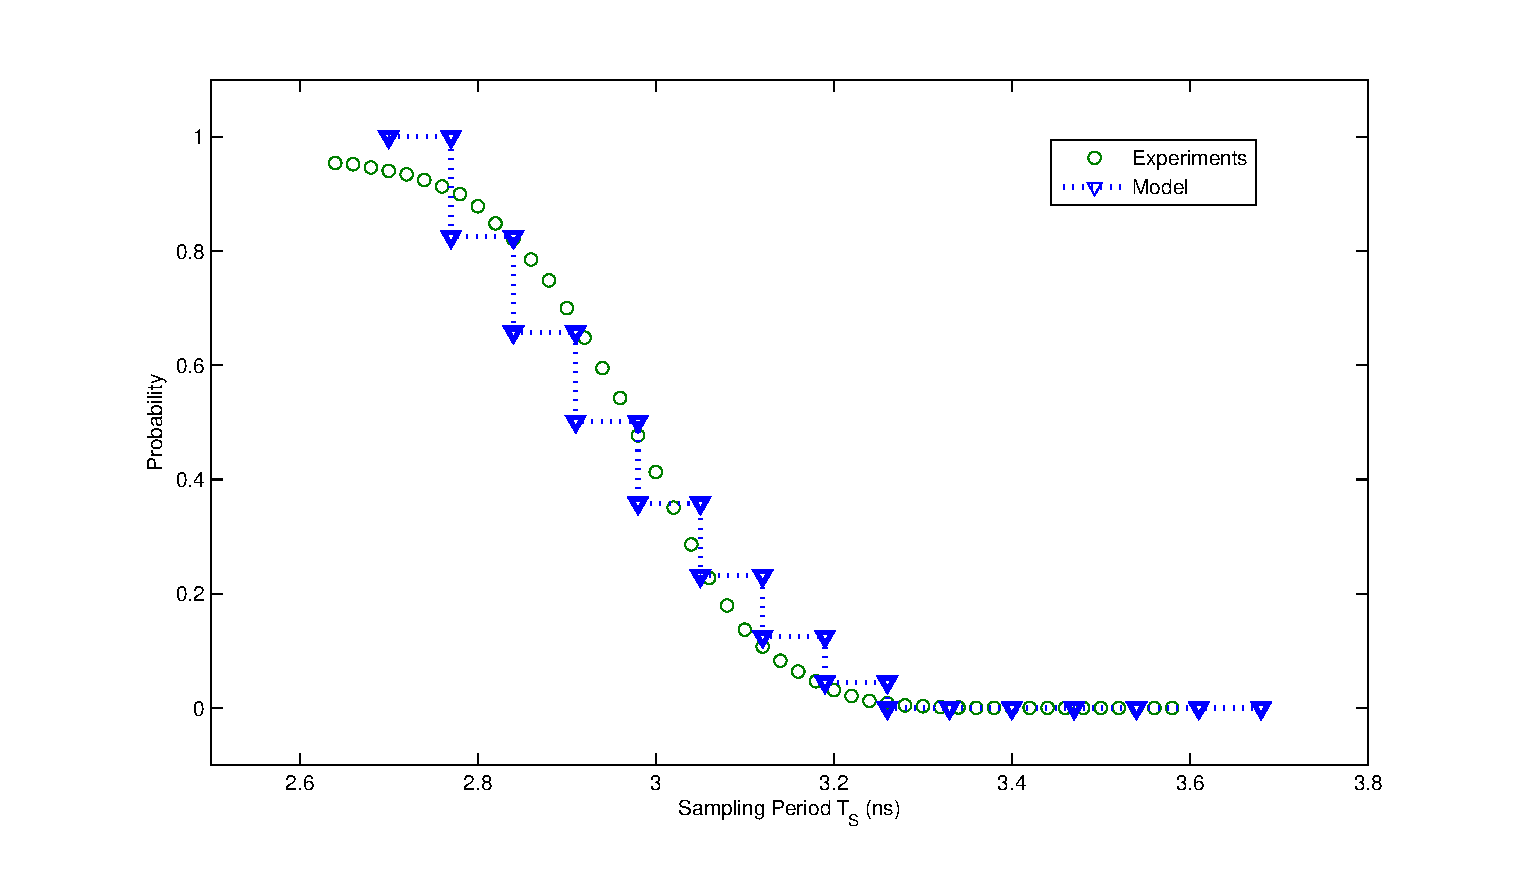
\includegraphics[width=9cm,height=4.5cm]{./Figures/probTimingViolationFPGA.eps}
\caption{ Probability of timing violation for $N=8$ and $\delta=3$ }
\label{Fig:ProbTimingViol}
\end{center}
\end{figure}

\subsection{Verification of Models for Error Magnitude}
We then verify the proposed models for the estimation of timing errors. Fig.~\ref{FigerrorC} shows the distribution of the error $\varepsilon$ on the FPGA results of the Algorithm 1 with input data uniformly distributed into the digit set $\{\overline{1},0,1\}$. \\

\begin{figure}[tbp]
	\centering
	\includegraphics[width=8cm,height=5cm]{./Figures/FigerrorC}
\caption{Distribution of overclocking errors with respect to a variety of sampling period. The Xlable should be ``Sampling period'', which varies from 2ns to 3.5ns, and the Ylabel is ``Error Values''. }
	\label{FigerrorC}
	
\end{figure}

Several slice through Fig.~\ref{FigerrorC} are presented in Fig.~\ref{Fig:gaussianOnlinedistr} for different sampling period values and the corresponding variances of overclocking errors. We observe that the profile of the error distribution changes as the value of the sampling period changes, and the width of the bell changes as well also (see Fig.~\ref{Fig:gaussianOnlinedistr}). The value of the mean is zero for all the values of the sampling period, while the variance of the distribution changes as the sampling period changes. In particular, the values of the variance decrease as the sampling period increases in agreement with the information provided by the values of the probability of timing violation.\\



\begin{figure}[tbp]
\centering
	\includegraphics[width=9cm,height=6cm]{./Figures/gaussianOnlinedistr}
	\caption{Several slice through Fig.~\ref{FigerrorC} that shows error distribution with respect to a variety of sampling periods and the corresponding variances of overclocking error. The results are obtained from experiments.}
	\label{Fig:gaussianOnlinedistr}
\end{figure}




We have compared these experimental results with the results provided by the model defined in (\ref{Eq:varfinal}). The Figure \ref{Error_Function_Spline_experiment} shows the curve provided by the model (blue line) and the experimental results (red stars). It can be seen that the modelled results are close to the experimental results. 

%the average of the values of the error obtained by comparing the two different values for each value of the sampling period is the $O(10^{-3})$. \\



\begin{figure}[tbp]
\centering
  \includegraphics[width=8cm,height=5cm]{./Figures/Error_Function_Spline_experiment}
  \caption{Variances of overclocking errors. The results are obtained from the proposed models (blue line) and the experiments (red stars). (Legend and xylabels to be added.) }\label{Error_Function_Spline_experiment}
\end{figure}




\section{Case Study: Image Filter}\label{Sec:CaseStudy}
\subsection{Experimental Setup}
The benefits of the proposed methodology are demonstrated by using a $3\times3$ Gaussian image filter, which is implemented with two types of computer arithmetic. One is the binary online arithmetic while the other is the binary traditional arithmetic. For design with online arithmetic, all inputs and outputs are represented in the online format as given in (\ref{Eq:Online_Operands}). The basic building blocks: adders and multipliers as described in Section~\ref{subsec:OnlineAdder} and Section~\ref{subsec:OnlineMultiplier} are employed. For design with traditional arithmetic, all signals are represented using the 2's complement format. We build this type of image filter by using speed-optimized adders and multipliers which are created using Xilinx Core Generator \cite{XilinxMult}. 

In order to achieve the desired latency between input and output, both designs are overclocked and the errors seen at the output are recorded. The results are obtained from a Xilinx Virtex-6 FPGA xxx through post place and route simulations. The results are evaluated in terms of mean relative error (MRE), which represents the percentage of error at outputs, as given by (\ref{Eq:MRE}) where $E_{error}$ and $E_{out}$ refer to the mean value of error and correct output, respectively.
%
\begin{eqnarray}\label{Eq:MRE}
\scriptsize
  MRE=\left|\frac{E_{error}}{E_{out}}\right|\times100\%
  %MRE=\left|{E_{error}}/{E_{out}}\right|\times100\%
\end{eqnarray}
\normalsize

In our experiments, two types of input data are utilized. One is randomly sampled from a uniform distribution of $N$-digit numbers. This type is referred to as ``Uniform Independent (UI) inputs''. The other is called ``real inputs'', which are the pixel values of several $512\times512$ benchmark images.

\subsection{Quantify the Impact of Overclocking}
The MRE values of the image filter with traditional arithmetic (dotted lines) and online arithmetic (solid lines) when $N=8$ are illustrated in Fig.~\ref{Fig:MRE_ImageFilter}. According to the timing analysis tool, the rated operating frequencies of the two designs are $169$MHz and $148$MHz, respectively. However as seen in Fig.~\ref{Fig:MRE_ImageFilter}, for the UI inputs, design with online arithmetic actually operates at a higher frequency without timing violations in comparison to the design using traditional arithmetic. This error-free frequency is even larger when using the real image data as inputs, since the real data do not exactly follow the uniform distribution or the independent assumption. In Fig.~\ref{Fig:MRE_ImageFilter} the ``Lena'' benchmark image is used as the real inputs.

\begin{figure}
    \centering
    \includegraphics[width=.48\textwidth]{./Figures/Exps/MRE.eps}
    %\vspace{-4ex}
    \caption{Overclocking error in an image filter with two types of computer arithmetic: online arithmetic and standard binary arithmetic, of which the rated frequencies are 148.3MHz and 168.7MHz, respectively, according to the timing analysis tool.}
    \label{Fig:MRE_ImageFilter}
    %\vspace{-3ex}
\end{figure}

If errors can be tolerated, we may allow timing violations to happen for better performance. The sensitivity of overclocking for a given arithmetic can be evaluated by the data slope in Figure~\ref{Fig:MRE_ImageFilter}. For instance under an error budget of $1\%$~MRE, using UI inputs the frequency speedup of the traditional design is $3.89\%$ with respect to the maximum frequency without errors, whereas the design with online arithmetic can be overclocked by $6.85\%$. This indicates that online arithmetic is less sensitive to overclocking, as discussed in Section~\ref{Sec:MeanError}. The difference is greater using real image data: $13.74\%$ frequency speedup with online arithmetic against $4.04\%$ with traditional arithmetic, because longer chains happen with a smaller probability with real inputs.
%\vspace{-1ex}

The output images for both design scenarios are presented in Fig.~\ref{Fig:LenaImage}. Since the overclocking errors are in the least significant ends of the results with online arithmetic, the degradation on the image can be hardly observed. In contrast, timing violations cause error in the MSDs with traditional arithmetic. This leads to ``salt and pepper noise'' and severe quality loss as shown on the images in the right column of Fig.~\ref{Fig:LenaImage}. Furthermore, errors in the MSDs result in large noise power. Hence the signal-to-noise ratio (SNR) of the traditional design is small.

\begin{figure}[htb]
  %\vspace{-2.5ex}
  \centering
  \subfigure[1.05$f_0$,~SNR=38.3dB]{
  \begin{minipage}[c]{0.24\textwidth}
    \centering
    \includegraphics[width=1.3in]{./Figures/Exps/Lena/Online_T404.eps}
  \end{minipage}%
  }% This is important! use % to indicate same line, otherwise new line
  \subfigure[1.05${f_0}'$,~SNR:21.5dB]{
  \begin{minipage}[c]{0.24\textwidth}
    \centering
    \includegraphics[width=1.3in]{./Figures/Exps/Lena/Trad_T426.eps}
  \end{minipage}
  }\vspace{-1ex}
  \subfigure[1.15$f_0$,~SNR:36.2dB]{
  \begin{minipage}[c]{0.24\textwidth}
    \centering
    \includegraphics[width=1.3in]{./Figures/Exps/Lena/Online_T370.eps}
  \end{minipage}
  }%
  \subfigure[1.15${f_0}'$,~SNR:9.0dB]{
  \begin{minipage}[c]{0.24\textwidth}
    \centering
    \includegraphics[width=1.3in]{./Figures/Exps/Lena/Trad_T390.eps}
  \end{minipage}
  }\vspace{-1ex}
  \subfigure[1.25$f_0$,~SNR:26.7dB]{
  \begin{minipage}[c]{0.24\textwidth}
    \centering
    \includegraphics[width=1.3in]{./Figures/Exps/Lena/Online_T340.eps}
  \end{minipage}%
  }% same line
  \subfigure[1.25${f_0}'$,~SNR:8.5dB]{
  \begin{minipage}[c]{0.24\textwidth}
    \centering
    \includegraphics[width=1.3in]{./Figures/Exps/Lena/Trad_T358.eps}
  \end{minipage}
  }
%\vspace{-2ex}
\caption{Output images of image filter using online arithmetic (left column) and traditional arithmetic (right column), where $f_0$ and ${f_0}'$ denote the maximum error-free frequencies for each design.}
\label{Fig:LenaImage}
%\vspace{-1ex}
\end{figure}


\subsection{Potential Benefits in Circuit Design}
In general, our results could be of interest to a circuit designers in two ways. By choosing different arithmetic and data representations, either a circuit can be designed to operate at a certain frequency with the minimum possible MRE, or a given error budget specified by the algorithm designer can be met with the fastest achievable frequency. For the first case, the experimental results obtained by UI inputs and 4 benchmark images are summarized in Table~\ref{Tab:MRE_Redu_Freq} in terms of the relative reduction of MRE as given by (\ref{Eq:MRE_Reduction}) where $MRE_{OL}$ and $MRE_{Trad}$ denote the value obtained with online arithmetic and with traditional arithmetic, respectively, and in Table \ref{Tab:SNR_Impro_Freq} for the differences of SNR.

We also perform experiments using other benchmark images. The results are summarized in Table~\ref{Tab:MRE_Redu_Freq} and Table~\ref{Tab:SNR_Impro_Freq} in terms of the relative reduction of MRE and the improvements of SNR, respectively. In both tables the frequency is normalized to the maximum error-free frequency for each arithmetic. From Table~\ref{Tab:MRE_Redu_Freq}, a significant reduction of MRE can be observed using online arithmetic. The geometric mean reduction of MRE is $89.2\%$ using UI data. Even larger reductions of MRE can be achieved when testing with real image data, varying from $97.3\%$ to $98.2\%$, as expected given the results shown in Figure~\ref{Fig:MRE_ImageFilter}. Similarly from Table~\ref{Tab:SNR_Impro_Freq}, the improvements in SNR are $21.4dB\sim43.9dB$.
%\vspace{-1ex}

\begin{eqnarray}\label{Eq:MRE_Reduction}
\scriptsize
  \frac{MRE_{Trad}-MRE_{OL}}{MRE_{Trad}}\times100\%
  %{(MRE_{Trad}-MRE_{OL})}/{MRE_{Trad}}\times100\%
\normalsize
\end{eqnarray}



\begin{table}[tbh]
\vspace{-1ex}
\renewcommand{\arraystretch}{1.1}
\setlength{\tabcolsep}{4.1pt}
\caption{Relative Reduction of MRE with Online Arithmetic for Various Normalized Frequencies.}
\vspace{1ex}
\label{Tab:MRE_Redu_Freq}
\small
%\scriptsize
\centering
\begin{tabular}{|c|ccccc|c|}
\hline
\multirow{2}*{\textbf{Inputs}} & \multicolumn{5}{c|}{\textbf{Normalized Frequency}} &
\multirow{2}*{\begin{tabular}{c}\textbf{Geo.}\\\textbf{Mean}\end{tabular}}\\
& 1.05 & 1.10 & 1.15 & 1.20 & 1.25 &\\
\hline
Uniform & 94.5\% & 89.1\% & 90.1\% & 88.3\% & 84.3\% & 89.2\%\\
Lena    & 99.3\% & 99.2\% & 98.9\% & 97.7\% & 94.9\% & 97.9\%\\
Pepper  & 99.7\% & 98.3\% & 98.1\% & 97.2\% & 95.1\% & 97.7\%\\
Sailboat& 99.5\% & 97.9\% & 97.3\% & 96.8\% & 95.1\% & 97.3\%\\
Tiffany & 99.9\% & 97.6\% & 98.4\% & 97.8\% & 97.2\% & 98.2\%\\
\hline
\end{tabular}
%\vspace{-1ex}
\normalsize
\end{table}

\begin{table}[thb]
%\vspace{-1ex}
\renewcommand{\arraystretch}{1.1}
\setlength{\tabcolsep}{4.1pt}
\caption{Improvement of SNR (dB) with Online Arithmetic for Various Normalized Frequencies.}
\vspace{1ex}
\label{Tab:SNR_Impro_Freq}
%\scriptsize
\small
\centering
\begin{tabular}{|c|ccccc|}
\hline
\multirow{2}*{\textbf{Inputs}} & \multicolumn{5}{c|}{\textbf{Normalized Frequency}} \\
& 1.05 & 1.10 & 1.15 & 1.20 & 1.25\\
\hline
Lena    & 44.6 & 36.3 & 33.2 & 29.1 & 22.9\\
Pepper  & 35.7 & 28.3 & 28.7 & 25.9 & 24.1\\
Sailboat& 33.7 & 27.5 & 26.3 & 25.0 & 21.7\\
Tiffany & 43.9 & 25.9 & 29.5 & 25.6 & 24.5\\
\hline
\end{tabular}
\vspace{-2ex}
\normalsize
\end{table}

For the second design perspective, Table~\ref{Tab:MRE_Reduc_Error} illustrates the frequency speedups with different input types when specific error budgets can be tolerated. We see that for all input types using online arithmetic still outperforms the traditional design for each MRE budget in terms of operating frequency. Likewise the geometric mean of frequency speed-ups is larger for real image inputs.\vspace{-1ex}

\begin{table}[tbh]
\vspace{-2ex}
\renewcommand{\arraystretch}{1.1}
\setlength{\tabcolsep}{4.1pt}
\caption{Relative Improvement in Frequency with Online Arithmetic for Various Error Budgets.}
\label{Tab:MRE_Reduc_Error}
\small
%\scriptsize
\centering
\begin{tabular}{|c|cccc|c|}
\hline
\multirow{2}*{\textbf{Inputs}} & \multicolumn{4}{c|}{\textbf{Error Budget}} &
\multirow{2}*{\begin{tabular}{c}\textbf{Geo.}\\\textbf{Mean}\end{tabular}}\\
& 0.01\% & 0.1\% & 1\% & 10\% &\\
\hline
Uniform & N/A & 4.59\%   & 8.78\%  & 12.83\% & 8.03\%\\
Lena    & 7.96\% & 11.50\%  & 16.39\% & 13.71\% & 11.88\%\\
Pepper  & 6.22\% & 8.87\%   & 18.68\% & 15.94\% & 11.32\%\\
Sailboat& 5.71\% & 8.87\%   & 16.93\% & 15.29\% & 10.70\%\\
Tiffany & 2.35\% & 6.90\%   & 18.58\% & 12.22\% & 7.79\% \\
\hline
\end{tabular}
\label{Tab:}
%\vspace{-2ex}
\normalsize
\end{table}

\subsection{Area Overhead of Our Approach}
The area comparison between two designs is illustrated in Table~\ref{Tab:AreaComparison}. While we notice that our approach comes at some increase in area, the FPGA architecture is optimized for conventional arithmetic. For instance, the Virtex series employs dedicated multiplexers and encoders for very fast ripple carry addition~\cite{Virtex6}. Besides, at least 2 orders of magnitude error reduction is obtained for a given frequency in our design, as shown in Figure \ref{Fig:MRE_ImageFilter}. Although the differences in both error and area can be compensated by using more digits with traditional arithmetic, this will result in longer delay and an even larger gap in frequency between two designs.

\begin{table}[tbh]
\vspace{-1ex}
\small
\caption{FPGA Resource Usage Comparison.}
\vspace{.5ex}
\centering
\label{Tab:AreaComparison}
\begin{tabular}{|c|cc|c|}
\hline
\multirow{2}*{\textbf{Metric}} & \multicolumn{2}{c|}{\textbf{Arithmetic Type}} &
\multirow{2}*{\textbf{Overhead}}\\
 & Traditional & Online &\\ \hline
 Look-Up Tables   & 912 & 1896 & 2.08 \\ \hline
 Slices & 324 & 525 & 1.62 \\ \hline

\end{tabular}
\vspace{-1ex}
\normalsize
\end{table}






























%\section*{Acknowledgment}




% Can use something like this to put references on a page
% by themselves when using endfloat and the captionsoff option.
\ifCLASSOPTIONcaptionsoff
  \newpage
\fi



% trigger a \newpage just before the given reference
% number - used to balance the columns on the last page
% adjust value as needed - may need to be readjusted if
% the document is modified later
%\IEEEtriggeratref{8}
% The "triggered" command can be changed if desired:
%\IEEEtriggercmd{\enlargethispage{-5in}}

% references section

% can use a bibliography generated by BibTeX as a .bbl file
% BibTeX documentation can be easily obtained at:
% http://www.ctan.org/tex-archive/biblio/bibtex/contrib/doc/
% The IEEEtran BibTeX style support page is at:
% http://www.michaelshell.org/tex/ieeetran/bibtex/
%\bibliographystyle{IEEEtran}
% argument is your BibTeX string definitions and bibliography database(s)
%\bibliography{IEEEabrv,../bib/paper}
%
% <OR> manually copy in the resultant .bbl file
% set second argument of \begin to the number of references
% (used to reserve space for the reference number labels box)
\begin{thebibliography}{1}

\bibitem{onlinearith} Datapath synthesis for overclocking: Online Arithmetic for Latency-Accuracy Trade-offs.
\bibitem{convol} J. B. Uspensky, Introduction to Mathematical Probability (New York: McGraw-Hill, 1937)
\bibitem{ross} Ross, Introduction to Probability Models, University of Southern California - Los Angeles (CA), 2010 ELSEVIER
\bibitem{spline} C. de Boor, A Practical Guide to Splines, Springer-Verlag, 1978.
\bibitem{kendall} Kendall E. Atkinson, On the order of convergence of natural cubic spline interpolation, SIAM Journal on Numerical Analysis, Vol 5 No 1, 1968


\bibitem{IEEEhowto:kopka}
H.~Kopka and P.~W. Daly, \emph{A Guide to \LaTeX}, 3rd~ed.\hskip 1em plus
  0.5em minus 0.4em\relax Harlow, England: Addison-Wesley, 1999.

\end{thebibliography}

% biography section
% 
% If you have an EPS/PDF photo (graphicx package needed) extra braces are
% needed around the contents of the optional argument to biography to prevent
% the LaTeX parser from getting confused when it sees the complicated
% \includegraphics command within an optional argument. (You could create
% your own custom macro containing the \includegraphics command to make things
% simpler here.)
%\begin{IEEEbiography}[{\includegraphics[width=1in,height=1.25in,clip,keepaspectratio]{mshell}}]{Michael Shell}
% or if you just want to reserve a space for a photo:

%\begin{IEEEbiography}{Michael Shell}
%Biography text here.
%\end{IEEEbiography}

% if you will not have a photo at all:
%\begin{IEEEbiographynophoto}{John Doe}
%Biography text here.
%\end{IEEEbiographynophoto}



%\vfill

% Can be used to pull up biographies so that the bottom of the last one
% is flush with the other column.
%\enlargethispage{-5in}



\end{document}


